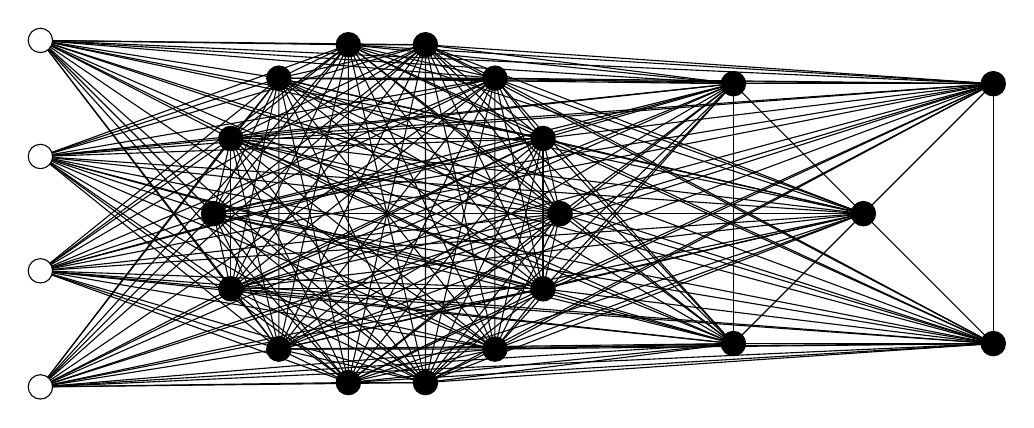
\begin{tikzpicture}[scale=2.2]
\def\a{3.5}
\def\b{1}
\def\c{0.5}

\foreach \s in {1,...,14}
{
	\coordinate (a\s) at ({\s*360/14}:1);
	\draw[fill=black] (a\s) circle (2pt);
};
\foreach \s in {1,...,13} {
	\foreach \t in {\s,...,14} {
		\draw (a\s) -- (a\t);
}; };

%\foreach\s in {1,...,4} {
%	\coordinate (b\s) at ({\s*360/4+45}:1.5);
%	\foreach \t in {1,...,14} {
%		\draw (b\s) -- (a\t);
%	};
%	\draw[fill=white] (b\s) circle (2pt);
%};

\coordinate (c1) at (2,0.75);
\coordinate (c2) at (2,-0.75);
\coordinate (c3) at (3.5,-0.75);
\coordinate (c4) at (3.5,0.75);
\coordinate (c5) at (2.75,0);

\draw (c1) -- (c2) -- (c3) -- (c4) -- (c1);
\draw (c1) -- (c3);
\draw (c2) -- (c4);

\foreach\s in {1,...,5} {
	\foreach \t in {1,...,14} {
		\draw (c\s) -- (a\t);
	};
	\draw[fill=black] (c\s) circle (2pt);
};

\coordinate (b1) at (-2,-1);
\coordinate (b2) at (-2,-0.33);
\coordinate (b3) at (-2,0.33);
\coordinate (b4) at (-2,1);

\foreach\s in {1,...,4} {
	\foreach \t in {1,...,14} {
		\draw (b\s) -- (a\t);
	};
	\foreach \t in {1,...,5} {
		\draw (c\t) -- (b\s);
	};
	\draw[fill=white] (b\s) circle (2pt);
};
\end{tikzpicture}